% ============================================================
%  YOLOv5 Object Detection — Beamer Presentation
%  AIMS Rwanda · Introduction to Neural Networks · March 2026
%  Group 3: Olusola T. Ogundepo, Lillian Mutesi,
%           Lucas M. Razafimanantsoa, Alliance Irigenera
% ============================================================
\documentclass[aspectratio=169,10pt]{beamer}

% ---------- theme -----------------------------------------------------------
\usetheme{Madrid}
\usecolortheme{seahorse}
\usefonttheme{professionalfonts}

% ---------- packages --------------------------------------------------------
\usepackage{graphicx}
\usepackage{booktabs}
\usepackage{amsmath,amssymb}
\usepackage{xcolor}
\usepackage{tikz}
\usetikzlibrary{shapes.geometric,arrows.meta,positioning,fit,backgrounds}
\usepackage{array}
\usepackage{multicol}
\usepackage{tcolorbox}
\tcbuselibrary{skins,breakable}
\usepackage{pifont}
\newcommand{\faUsers}{$\bigstar$}
\newcommand{\faCircle}[1][]{$\bullet$}
\newcommand{\faUser}{Pers.}
\newcommand{\faDog}{Dog}
\newcommand{\faCheckCircle}{\checkmark}
\newcommand{\faTimesCircle}{\ding{55}}
\usepackage{calc}

% ---------- colour palette --------------------------------------------------
\definecolor{navyblue}{HTML}{1A237E}
\definecolor{medblue} {HTML}{283593}
\definecolor{accent}  {HTML}{42A5F5}
\definecolor{lightbg} {HTML}{EEF2FF}
\definecolor{vgreen}  {HTML}{2E7D32}
\definecolor{vred}    {HTML}{C62828}
\definecolor{vorange} {HTML}{E65100}

% ---------- beamer colours --------------------------------------------------
\setbeamercolor{palette primary}  {bg=navyblue,fg=white}
\setbeamercolor{palette secondary}{bg=medblue, fg=white}
\setbeamercolor{palette tertiary} {bg=accent,  fg=navyblue}
\setbeamercolor{palette quaternary}{bg=navyblue,fg=white}
\setbeamercolor{structure}        {fg=navyblue}
\setbeamercolor{block title}      {bg=navyblue,fg=white}
\setbeamercolor{block body}       {bg=lightbg}
\setbeamercolor{block title alerted}{bg=vred,fg=white}
\setbeamercolor{block body alerted}{bg=vred!10}
\setbeamercolor{block title example}{bg=vgreen,fg=white}
\setbeamercolor{block body example} {bg=vgreen!10}
\setbeamercolor{frametitle}       {bg=navyblue,fg=white}
\setbeamercolor{title}            {fg=white}
\setbeamercolor{subtitle}         {fg=accent}
\setbeamercolor{author}           {fg=white}
\setbeamercolor{institute}        {fg=lightbg}
\setbeamercolor{date}             {fg=lightbg}
\setbeamerfont{frametitle}        {size=\large,series=\bfseries}
\setbeamerfont{title}             {size=\Large,series=\bfseries}
\setbeamertemplate{navigation symbols}{}
\setbeamertemplate{caption}[numbered]

% ---------- tcolorbox shortcuts ---------------------------------------------
\tcbset{
  mybox/.style={
    enhanced, colback=lightbg, colframe=navyblue,
    boxrule=0.8pt, arc=4pt, fonttitle=\bfseries\small,
    coltitle=white, attach boxed title to top left={yshift=-2mm,xshift=4mm},
    boxed title style={colback=navyblue, arc=3pt}
  },
  greenbox/.style={mybox, colframe=vgreen, boxed title style={colback=vgreen}},
  redbox/.style={mybox, colframe=vred, boxed title style={colback=vred}},
}

% ---------- metadata --------------------------------------------------------
\title{Object Detection with YOLOv5}
\subtitle{on the Pascal VOC 2012 Dataset}
\author[Group 3]{%
  Olusola T.\ Ogundepo \and Lillian Mutesi \and
  Lucas M.\ Razafimanantsoa \and Alliance Irigenera}
\institute[AIMS Rwanda]{%
  African Institute for Mathematical Sciences, Kigali\\
  Introduction to Neural Networks}
\date{March 2026}

% ============================================================
\begin{document}
% ============================================================

% ── Title slide ──────────────────────────────────────────────────────────────
\begin{frame}[plain]
  \begin{tikzpicture}[remember picture, overlay]
    \fill[navyblue] (current page.north west) rectangle (current page.south east);
    \fill[medblue]  ([xshift=6.5cm]current page.north west)
                    rectangle (current page.south east);
    \fill[accent]   ([xshift=6.5cm,yshift=-0.05cm]current page.north west)
                    rectangle
                    ([xshift=6.55cm]current page.south west);
  \end{tikzpicture}
  \vspace{1.2cm}
  \begin{columns}[c]
    \column{0.56\textwidth}
      {\color{white}\bfseries\LARGE Object Detection\\[4pt]
       \color{accent}\bfseries\LARGE with YOLOv5}\\[6pt]
      {\color{lightbg}\large on the Pascal VOC 2012 Dataset}\\[10pt]
      \textcolor{accent}{\rule{5cm}{0.8pt}}\\[6pt]
      {\color{lightbg!80!white}\small Introduction to Neural Networks\\
       AIMS Rwanda, Kigali }
    \column{0.40\textwidth}
      \begin{tcolorbox}[enhanced, colback=navyblue!60!black,
                        colframe=accent, arc=5pt, boxrule=0.8pt,
                        title={\faUsers~Group 3}]
        \footnotesize\color{white}
        \faCircle[regular]~Olusola Timothy\ Ogundepo\\[2pt]
        \faCircle[regular]~Lillian Mutesi\\[2pt]
        \faCircle[regular]~Lucas M.\ Razafimanantsoa\\[2pt]
        \faCircle[regular]~Alliance Irigenera
      \end{tcolorbox}
  \end{columns}
\end{frame}

% ── Outline ──────────────────────────────────────────────────────────────────
\begin{frame}{Outline}
  \tableofcontents[hideallsubsections]
\end{frame}

% ============================================================
\section{Task Description}
% ============================================================
\begin{frame}{Task Description }
  \begin{columns}[T]
    \column{0.48\textwidth}
      \begin{block}{What is Object Detection?}
        \begin{itemize}\setlength\itemsep{3pt}
          \item Identify \& localise objects in an image
          \item Output: \textbf{class label} + \textbf{bounding box}
          \item Combines classification and regression
          \item Evaluated with IoU 
        \end{itemize}
      \end{block}
      \vspace{4pt}
      \begin{exampleblock}{Our Goal}
        Train \textbf{YOLOv5} on Pascal VOC 2012 (20 classes)
        to accurately detect \& classify objects in
        images.
      \end{exampleblock}
      \vspace{4pt}
      \begin{tcolorbox}[enhanced, colback=navyblue, colframe=navyblue,
                        arc=3pt, boxrule=0pt]
        \centering\color{accent}\bfseries
        $\mathrm{Confidence} = P(\text{object})\times\mathrm{IoU}$
      \end{tcolorbox}

    \column{0.50\textwidth}
      \centering
      % ── IoU diagram via TikZ ──────────────────────────────
      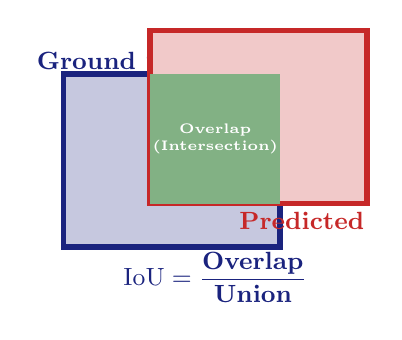
\begin{tikzpicture}[scale=0.55]
        % GT box
        \fill[navyblue!25] (0,0) rectangle (5,4);
        \draw[navyblue,line width=2pt] (0,0) rectangle (5,4);
        \node[navyblue,font=\bfseries\small] at (1.5,4.3) {Ground Truth};
        % Pred box
        \fill[vred!25] (2,1) rectangle (7,5);
        \draw[vred,line width=2pt] (2,1) rectangle (7,5);
        \node[vred,font=\bfseries\small] at (5.5,0.6) {Predicted};
        % Intersection
        \fill[vgreen!60] (2,1) rectangle (5,4);
        \node[white,font=\bfseries\tiny,align=center] at (3.5,2.5)
              {Overlap\\(Intersection)};
        % formula
        \node[font=\bfseries\small,navyblue] at (3.5,-0.7)
          {$\displaystyle\mathrm{IoU}=\frac{\text{Overlap}}{\text{Union}}$};
      \end{tikzpicture}
      \vspace{4pt}

      % ── Pipeline arrows ───────────────────────────────────
      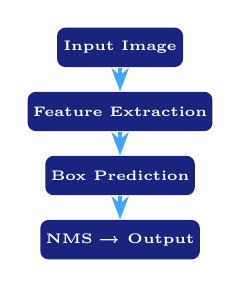
\begin{tikzpicture}[
        box/.style={rectangle,rounded corners=3pt,fill=navyblue,
                    text=white,font=\bfseries\tiny,
                    minimum width=1.6cm,minimum height=0.5cm,
                    inner sep=2pt},
        arr/.style={-Stealth,accent,line width=1.2pt},
        node distance=0.3cm]
        \node[box] (inp) {Input Image};
        \node[box,below=of inp] (feat) {Feature Extraction};
        \node[box,below=of feat] (bbox) {Box Prediction};
        \node[box,below=of bbox] (nms) {NMS → Output};
        \draw[arr] (inp)--(feat);
        \draw[arr] (feat)--(bbox);
        \draw[arr] (bbox)--(nms);
      \end{tikzpicture}
  \end{columns}
\end{frame}

% ============================================================
\section{Dataset}
% ============================================================
\begin{frame}{Dataset — Pascal VOC 2012}
  \begin{columns}[T]
    \column{0.45\textwidth}
      \begin{block}{Pascal VOC 2012}
        \begin{itemize}\setlength\itemsep{2pt}
          \item Benchmark for detection \& segmentation
          \item Real-world photographs, 20 object classes
          \item YOLO-format annotations:\\
                \texttt{class xc yc w h} (normalised to [0,1])
        \end{itemize}
      \end{block}
      \vspace{6pt}
      \vspace{4pt}
      \begin{alertblock}{Class Imbalance}
        \textbf{Class imbalance:} Person class appears significantly more frequently than others\\
      \end{alertblock}

    \column{0.52\textwidth}
      \begin{figure}
        \centering
        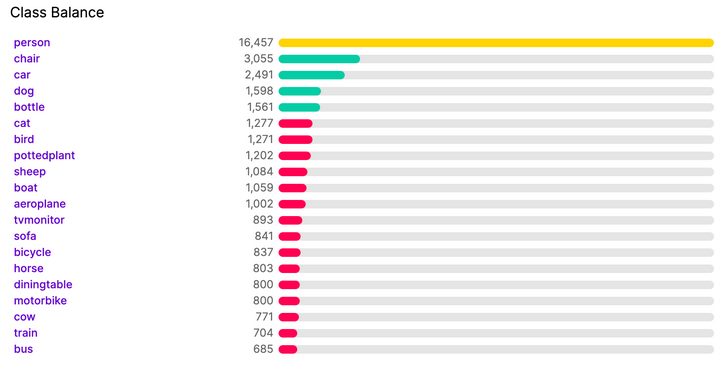
\includegraphics[width=\linewidth]{../Images/imbalance.png}
        \caption{Class distribution in Pascal VOC 2012 training subset}
      \end{figure}
  \end{columns}
\end{frame}

% ============================================================
\section{Algorithm Description — YOLOv5}
% ============================================================

% ── YOLO Concepts ────────────────────────────────────────────────────────────
\begin{frame}{Algorithm — You Only Look Once (YOLO)}
  \begin{block}{Core Idea}
    YOLO reformulates detection as a \textbf{single regression problem}:
    one forward pass predicts all bounding boxes \& class probabilities simultaneously.
  \end{block}
  \vspace{4pt}
  \begin{columns}[T]
    \column{0.33\textwidth}
      \begin{tcolorbox}[mybox, title={Grid}]
        \footnotesize
        Image divided into $S\times S$ cells.\\
        Each cell detects objects whose \textbf{centre} falls within it.
      \end{tcolorbox}
      \vspace{3pt}
      \begin{tcolorbox}[mybox, title={Bounding Box}]
        \footnotesize
        $(x_c,y_c,w,h)$: centre + dimensions,\\
        normalised to $[0,1]$.
      \end{tcolorbox}
    \column{0.33\textwidth}
      \begin{tcolorbox}[mybox, title={Confidence Score}]
        \footnotesize
        $\text{Conf}=P(\text{obj})\times\mathrm{IoU}$\\[2pt]
        Measures presence AND accuracy.
      \end{tcolorbox}
      \vspace{3pt}
      \begin{tcolorbox}[mybox, title={Class Probability}]
        \footnotesize
        Each cell predicts\\
        $P(\text{class}_i\mid\text{object})$\\
        for all $C$ classes.
      \end{tcolorbox}
    \column{0.30\textwidth}
      \begin{tcolorbox}[mybox, title={NMS}]
        \footnotesize
        Non-Maximum Suppression removes duplicate detections.\\
        Keeps highest-confidence box per object.
      \end{tcolorbox}
      \vspace{3pt}
      \begin{tcolorbox}[greenbox, title={Speed}]
        \footnotesize
        Single forward pass\\
        $\Rightarrow$ real-time detection.\\
        No region proposals needed.
      \end{tcolorbox}
  \end{columns}
\end{frame}

% ── YOLOv5 Architecture ───────────────────────────────────────────────────────
\begin{frame}{YOLO Algorithm Illustration}
  \begin{figure}
    \centering
    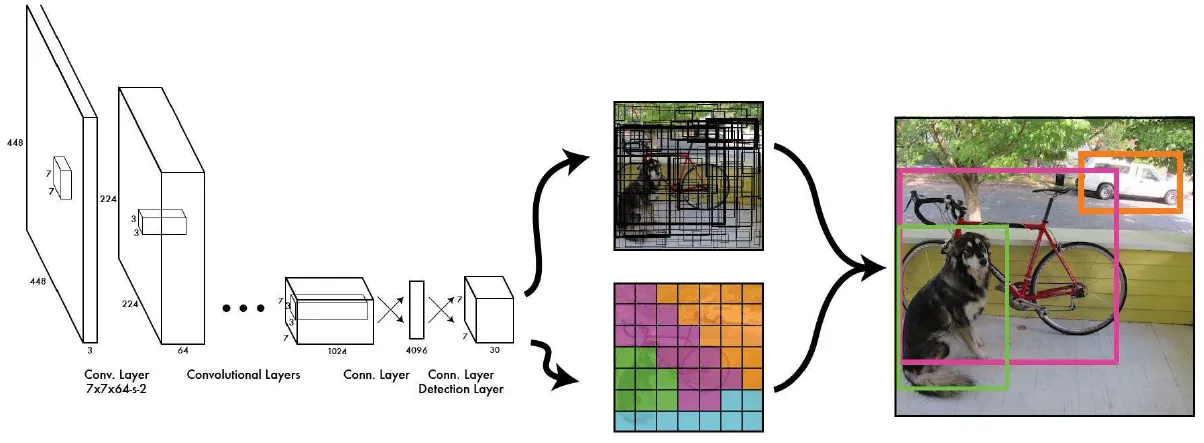
\includegraphics[width=0.96\linewidth]{../Images/yolo_algo.png}
    \caption{YOLO single-pass detection pipeline: grid division, box prediction, and NMS}
  \end{figure}
\end{frame}



% ── Detection Result: Person + Dog ───────────────────────────────────────────
\begin{frame}{Example of Detection Output}
  \begin{columns}[c]
    \column{0.62\textwidth}
      \begin{figure}
        \centering
        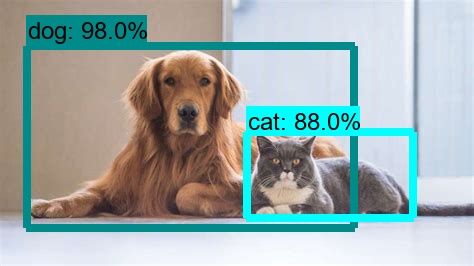
\includegraphics[width=\linewidth]{../Images/detection.png}
        \caption{Sample detection output from our trained YOLOv5 model}
      \end{figure}
    \column{0.36\textwidth}
      \begin{tcolorbox}[redbox, title={Dog}]
        \footnotesize
        \textbf{Confidence:} 0.98\\[3pt]
      \end{tcolorbox}
      \vspace{6pt}
      \begin{tcolorbox}[greenbox, title={Cat}]
        \footnotesize
        \textbf{Confidence:} 0.88\\[3pt]
      \end{tcolorbox}
      \vspace{6pt}
     
  \end{columns}
\end{frame}

% ============================================================
\section{Model Training}
% ============================================================


\begin{frame}{Model Training}
\begin{columns}[T]
\begin{column}{0.48\textwidth}
  \begin{block}{Hyperparameters}
    \begin{tabular}{ll}
      Image size    & $128 \times 128$ px \\[3pt]
      Batch size    & 8                   \\[3pt]
      Epochs        & 10                  \\[3pt]
      Optimiser     & Adam                \\[3pt]
      Learning rate & $10^{-3}$           \\[3pt]
      Subset size   & 500 images          \\[3pt]
      Device        & CPU                 \\
    \end{tabular}
  \end{block}

  \vspace{0.1cm}
  \textbf{Target encoding (\texttt{encode\_targets}):}\\
  Each ground-truth box is placed into the grid cell
  whose centre falls within it. The target tensor has
  shape $[S, S, B{\times}(5{+}C)]$.
\end{column}
\begin{column}{0.50\textwidth}
  \textbf{Training loop per batch:}
  \begin{enumerate}
    \item Load batch of images + labels
    \item Resize to $128\times128$
    \item Encode ground-truth into $8\times8\times75$ tensor
    \item Forward pass through \texttt{YOLODetector}
    \item Compute \texttt{yolo\_loss}
    \item \texttt{loss.backward()} + \texttt{optimizer.step()}
    \item Record epoch average loss
  \end{enumerate}

  \vspace{0.1cm}
  Model weights saved to \texttt{yolo\_voc.pt} after training.\\[4pt]
  Seed fixed at $42$ for reproducibility.
\end{column}
\end{columns}
\end{frame}


% ============================================================
\section{Results \& Evaluation}
% ============================================================

\begin{frame}{Training Loss Curve}
\begin{columns}[T]
\begin{column}{0.60\textwidth}
\begin{figure}
    \centering
    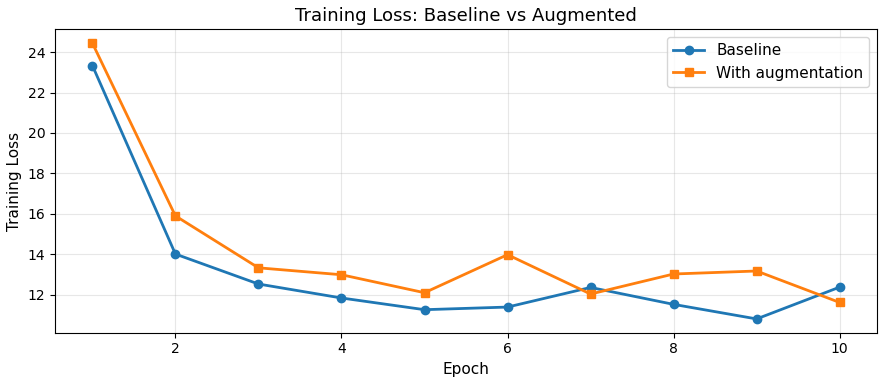
\includegraphics[width=1.0\linewidth]{../Images/loss_compare.png}
    \caption{Training Loss: Baseline vs Augmented}
    \label{fig:placeholder}
\end{figure}
\end{column}
\begin{column}{0.38\textwidth}
  \begin{block}{Baseline Summary}
    \begin{itemize}
      \item Start: \textbf{23.34}
      \item Final: \textbf{12.38}
      \item Reduction: \textbf{47.0\%}
    \end{itemize}
  \end{block}

  \vspace{0.1cm}
  \textbf{Observations:}
  \begin{itemize}
    \item Steep drop epochs 1–3\\
      (model learns basics)
    \item Oscillation from epoch 5\\
      (small batch size = 8)
    \item Aug.~model starts higher\\
      (harder, varied inputs)
    \item Both converge to\\
      similar final loss
  \end{itemize}
\end{column}
\end{columns}
\end{frame}














\begin{frame}{Evaluation Metrics}
  \begin{columns}[T]
    \column{0.48\textwidth}
       \begin{block}{Loss Function}
\footnotesize
\[
\mathcal{L}
=
\lambda_{\text{coord}} \mathcal{L}_{xy}
+
\lambda_{\text{coord}} \mathcal{L}_{wh}
+
\mathcal{L}_{\text{obj}}
+
\lambda_{\text{noobj}} \mathcal{L}_{\text{noobj}}
+
\mathcal{L}_{\text{cls}}
\]

\begin{itemize}\setlength\itemsep{2pt}
    \item \textbf{Coordinate loss}:
    squared error on predicted box centre $(x,y)$, applied only to cells containing an object.
    
    \item \textbf{Width/height loss}:
    squared error on $\sqrt{w}$ and $\sqrt{h}$, giving less sensitivity to large boxes.
    
    \item \textbf{Object confidence loss}:
    squared error for cells that contain an object.
    
    \item \textbf{No-object loss}:
    squared error on confidence for empty cells, weighted by $\lambda_{\text{noobj}}$.
    
    \item \textbf{Class loss}:
    squared error on class predictions, computed only for cells containing an object.
\end{itemize}
\end{block}

    \column{0.48\textwidth}
      \begin{block}{Results }
        \footnotesize
        \begin{tabular}{lc}
          \toprule
          \textbf{Set}       & \textbf{Mean YOLO Loss}\\
          \midrule
          Training subset              & $\approx 12.4128$\\
          Validation (full)             & $\approx 12.6849$\\
          \midrule
          Training subset (augmented)   & $\approx 11.1727$\\
          Validation (augmented)        & $\approx 13.2454$\\
          \bottomrule
        \end{tabular}
      \end{block}
      \vspace{4pt}
      \end{columns}
\end{frame}





%% ===========================================================
\section{Advanced Study: Data Augmentation}
%% ===========================================================

\begin{frame}{Advanced Study: Data Augmentation}
\begin{columns}[T]
\begin{column}{0.50\textwidth}
  \begin{block}{Motivation}
    With only 500 training images the model can memorise
    specific pixel patterns. Augmentation introduces
    controlled variation at load time.
  \end{block}

  \vspace{0.1cm}
  \textbf{Transforms applied:}
  \begin{itemize}
    \item \texttt{RandomHorizontalFlip}$(p=0.5)$
    \item \texttt{ColorJitter}(brightness$=0.3$, contrast$=0.3$, saturation$=0.2$)
    \item \texttt{RandomRotation}(degrees$=10$)
  \end{itemize}

  \vspace{0.1cm}
  \textbf{Experimental design:}\\
  Train a \textbf{second model} (\texttt{model\_aug}) from scratch;
  same architecture, same hyperparameters, same 500 images,
  only the transform pipeline differs.
\end{column}
\begin{column}{0.47\textwidth}
  \begin{alertblock}{Known Limitation}
    \textbf{Horizontal flip mismatch:}\\[4pt]
    The flip is applied to the \emph{pixel tensor} only.
    The bounding-box coordinates are \textbf{not mirrored}
    $(c_x \not\to 1-c_x)$.\\[4pt]
    This introduces a label mismatch for $\approx$50\% of
    augmented samples.\\[4pt]
    Despite this, colour jitter and rotation still provide
    useful diversity; the experiment is a valid
    \textit{proof-of-concept}.\\[4pt]
    A correct fix: pass image \emph{and} boxes together
    through a joint augmentation pipeline.
  \end{alertblock}
\end{column}
\end{columns}
\end{frame}




% ============================================================
\section{Advantages \& Limitations}
% ============================================================
\begin{frame}{Advantages \& Limitations of YOLOv5}
  \begin{columns}[T]
    \column{0.48\textwidth}
      \begin{exampleblock}{Advantages}
        \footnotesize
        \begin{itemize}\setlength\itemsep{2pt}
          \item \textbf{Real-time}: single forward pass, faster than region-based methods
          \item \textbf{Global reasoning}: processes entire image; captures context, fewer false positives
          \item \textbf{End-to-end}: single regression problem, no multi-stage complexity
        \end{itemize}
      \end{exampleblock}
    \column{0.48\textwidth}
      \begin{alertblock}{Limitations}
       
\begin{itemize}
  \item \textbf{Small subset}: 500 of 13,690 images; weak generalisation
      \item \textbf{Low resolution} ($128\times128$); misses small objects
      \item \textbf{CPU only} (no GPU); forced simpler architecture
      \item \textbf{Only 10 epochs}; model did not fully converge
      \item \textbf{Flip-box mismatch}: corrupts $\sim$50\% of aug.\ labels
      \item \textbf{Class imbalance}: person dominates; biased detections
      \item \textbf{Loss-only eval}: no mAP reported
\end{itemize}
      \end{alertblock}
  \end{columns}
\end{frame}

%---------------------------








\begin{frame}{Possible Improvements}
  \begin{block}{}
    \begin{enumerate}\setlength\itemsep{4pt}
      \item Train on \textbf{all 13,690} images
      \item \textbf{GPU} + higher resolution ($416\times416$)
      \item \textbf{Fix horizontal flip}: mirror $c_x \to 1-c_x$ with joint image+box transform
      \item \textbf{Anchor clustering} via k-means on ground-truth boxes
      \item \textbf{LR scheduler} (e.g.\ cosine annealing)
      \item Report \textbf{mAP@0.5} for standard benchmark comparison
      \item \textbf{Focal loss} to address class imbalance
      \item \textbf{Transfer learning} from a pretrained backbone
    \end{enumerate}
  \end{block}
\end{frame}
% ── Conclusion ───────────────────────────────────────────────────────────────
\begin{frame}{Conclusion}
 
      \begin{block}{Summary}
        \begin{itemize}
      \item  Built a \textbf{YOLO detector from scratch}
        in PyTorch (backbone, head, loss function)
      \item Trained on Pascal VOC 2012 (20 classes)
        with a 500-image subset
      \item  Loss reduced by \textbf{47\%} over 10 epochs
        (23.34 $\to$ 12.38)
      \item  Conducted a \textbf{data augmentation study}
        with a second model for comparison
      \item Honestly discussed all limitations and
        proposed concrete improvements
    \end{itemize}
      \end{block}
      \vspace{4pt}
      \vspace{0.1cm}
  \textit{YOLO's strength is speed and end-to-end simplicity; scaling to
  full data with GPU training would close the accuracy gap.}
  \vspace{4pt}
  \begin{center}
    \large\color{navyblue}\bfseries Thank you! \quad Questions welcome.
  \end{center}
\end{frame}





 

\end{document}